\section{Adaptive dynamics: Can actions of accreted globular clusters constrain the gravitational potential?}
\subsection{Integrals of motion}

\subsubsection{Energy and angular momentum}
\subsubsection{Actions}
\subsection{Merger tree}
figure: Merger tree of Auriga 24. 
\subsection{Globular cluster sample selection}
\\figure: Selected CG particles in snapshot before merger and in \textit{z} = 0 snapshot.

\begin{figure}[htbp]
    \centering
    \begin{subfigure}[c]{0.45\textwidth}
    \centering
    	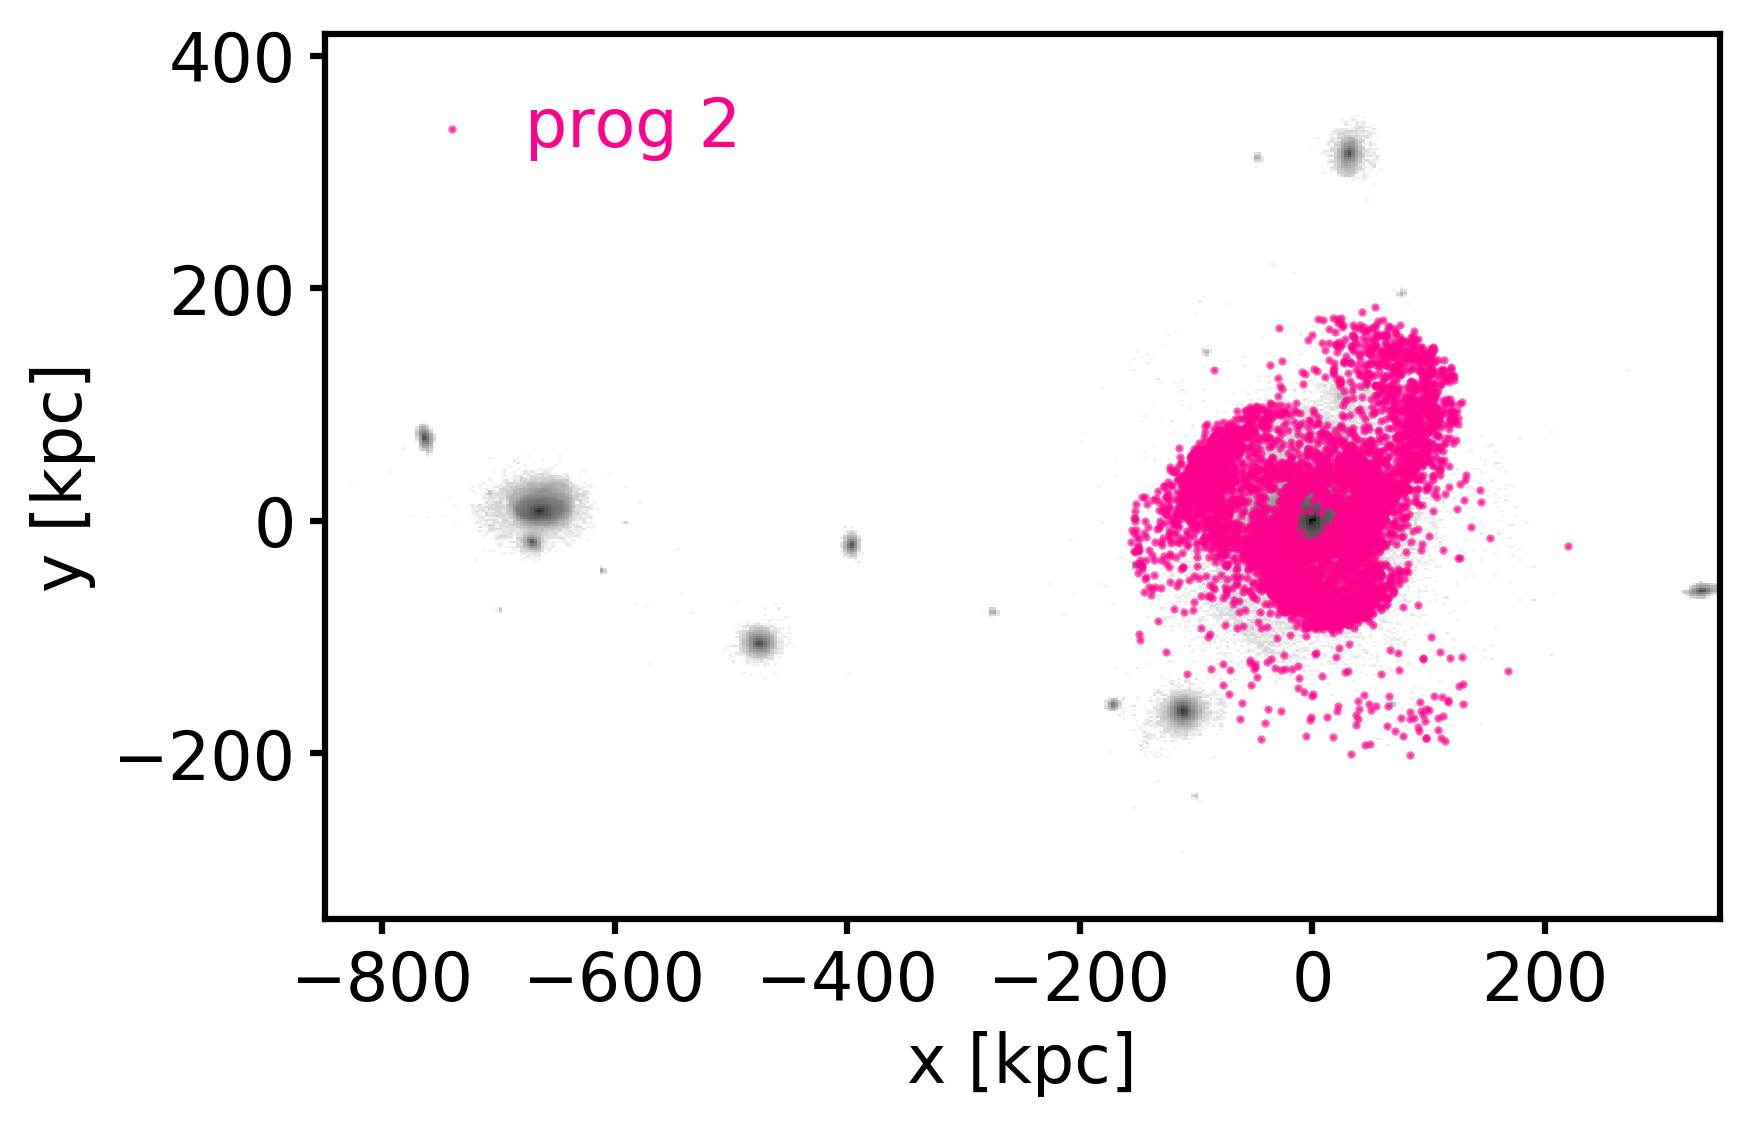
\includegraphics[width=\textwidth]{plots/Dynamics/dist/xy_dist_selected_GCs_prog_2_snap_127.png}
    	\label{fig:prog2_xy}
    \end{subfigure}
    ~ %add desired spacing between images, e. g. ~, \quad, \qquad, \hfill etc. 
    %(or a blank line to force the subfigure onto a new line)
    \begin{subfigure}[c]{0.45\textwidth}
        \centering
    	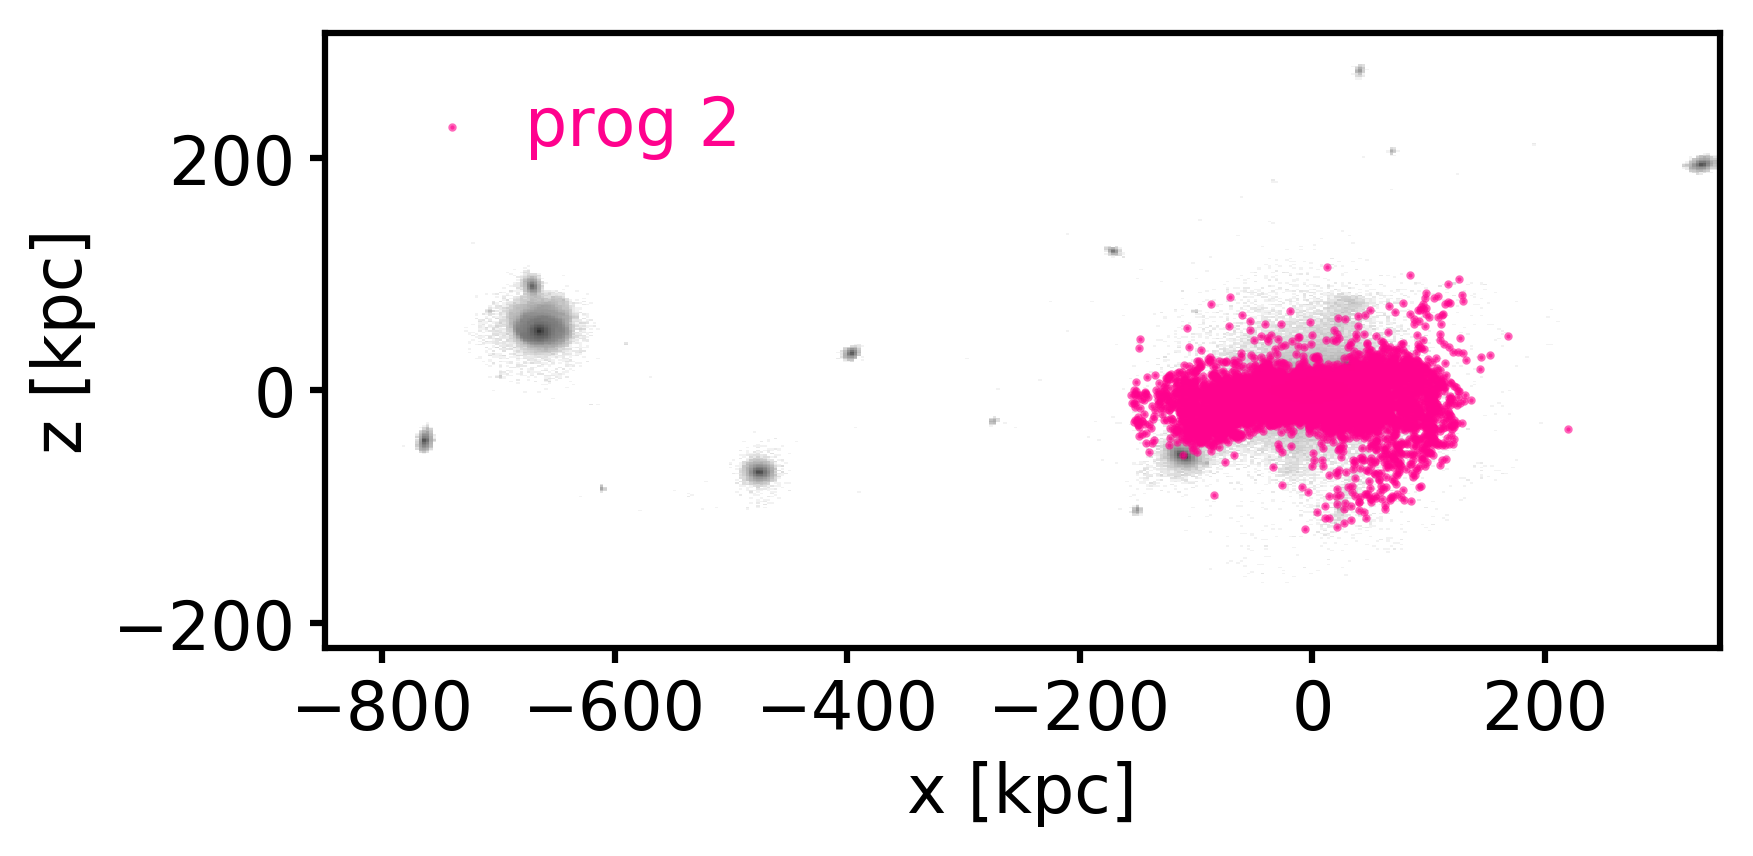
\includegraphics[width=\textwidth]{plots/Dynamics/dist/xz_dist_selected_GCs_prog_2_snap_127.png}
	    \label{fig:prog2_xz}
    \end{subfigure}
    
    \begin{subfigure}[c]{0.45\textwidth}
    \centering
    	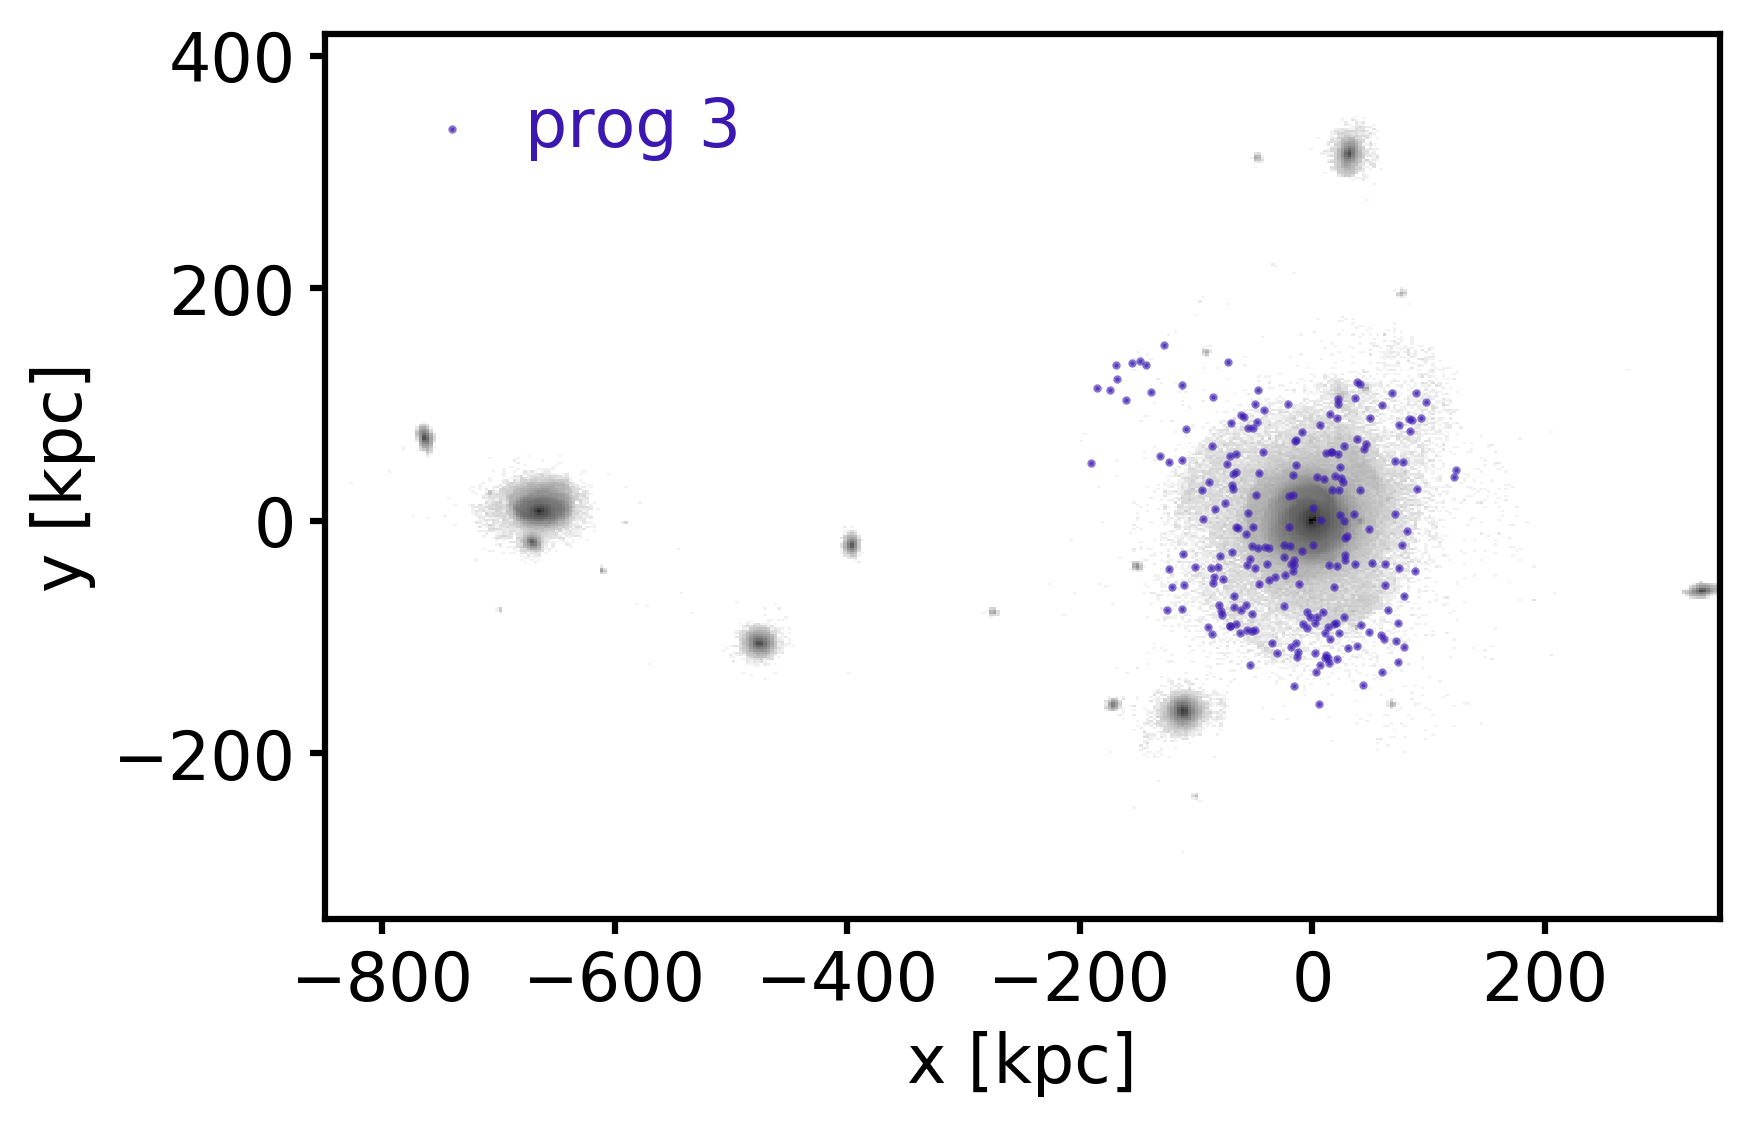
\includegraphics[width=\textwidth]{plots/Dynamics/dist/xy_dist_selected_GCs_prog_3_snap_127.png}
    	\label{fig:prog3_xy}
    \end{subfigure}
    ~ %add desired spacing between images, e. g. ~, \quad, \qquad, \hfill etc. 
    %(or a blank line to force the subfigure onto a new line)
    \begin{subfigure}[c]{0.45\textwidth}
        \centering
    	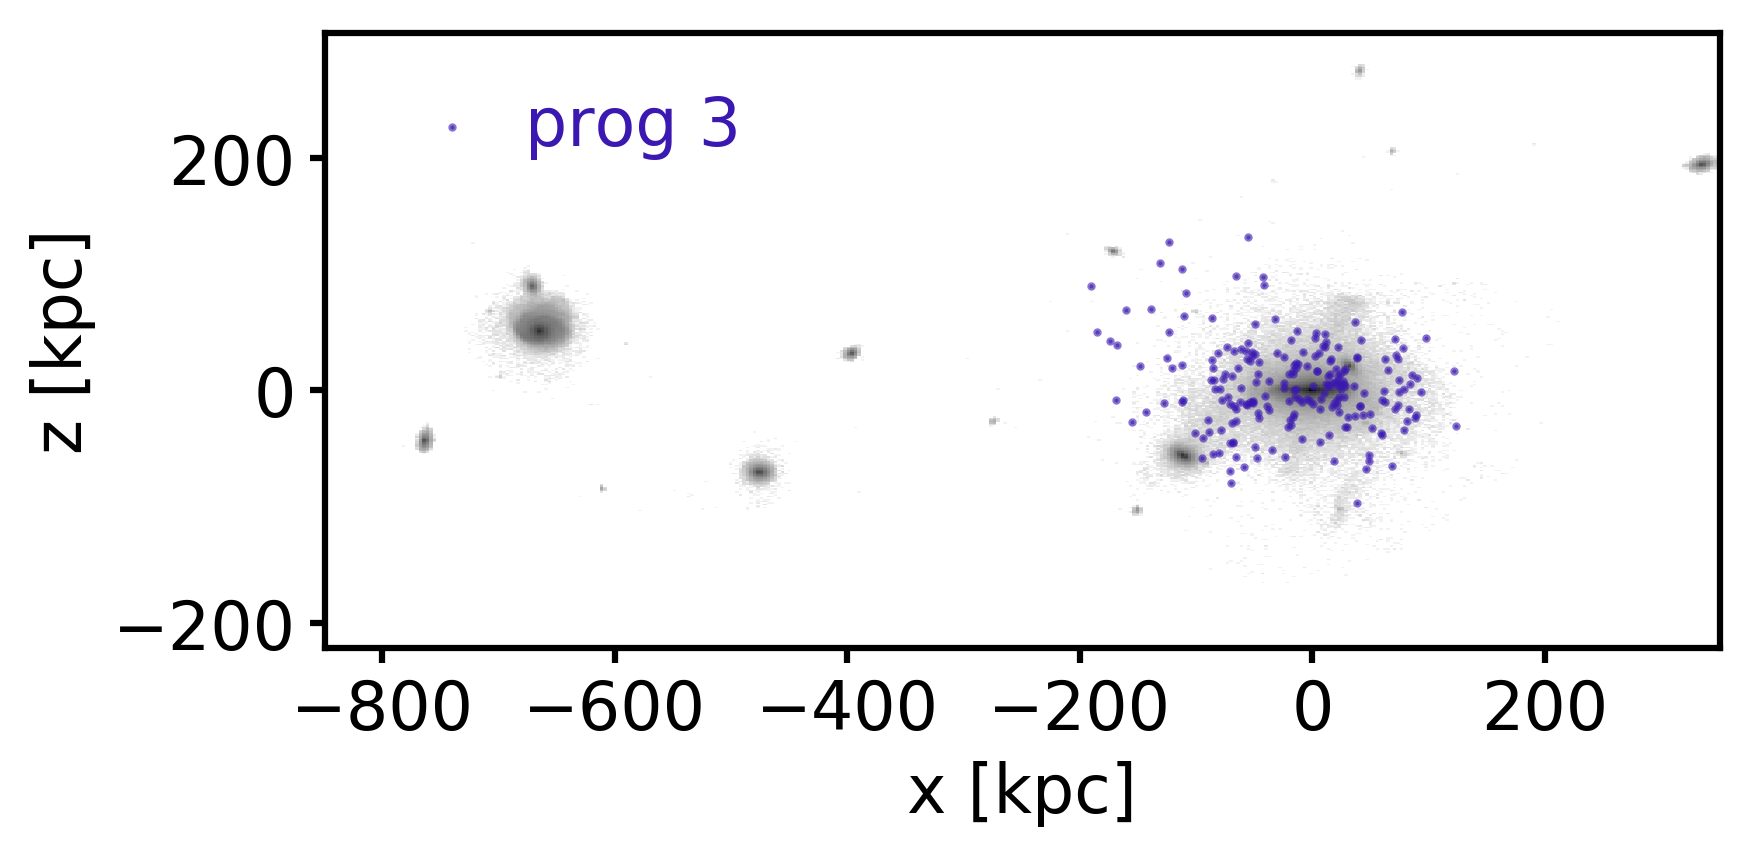
\includegraphics[width=\textwidth]{plots/Dynamics/dist/xz_dist_selected_GCs_prog_3_snap_127.png}
	    \label{fig:prog3_xz}
    \end{subfigure}
    
    \begin{subfigure}[c]{0.45\textwidth}
    \centering
    	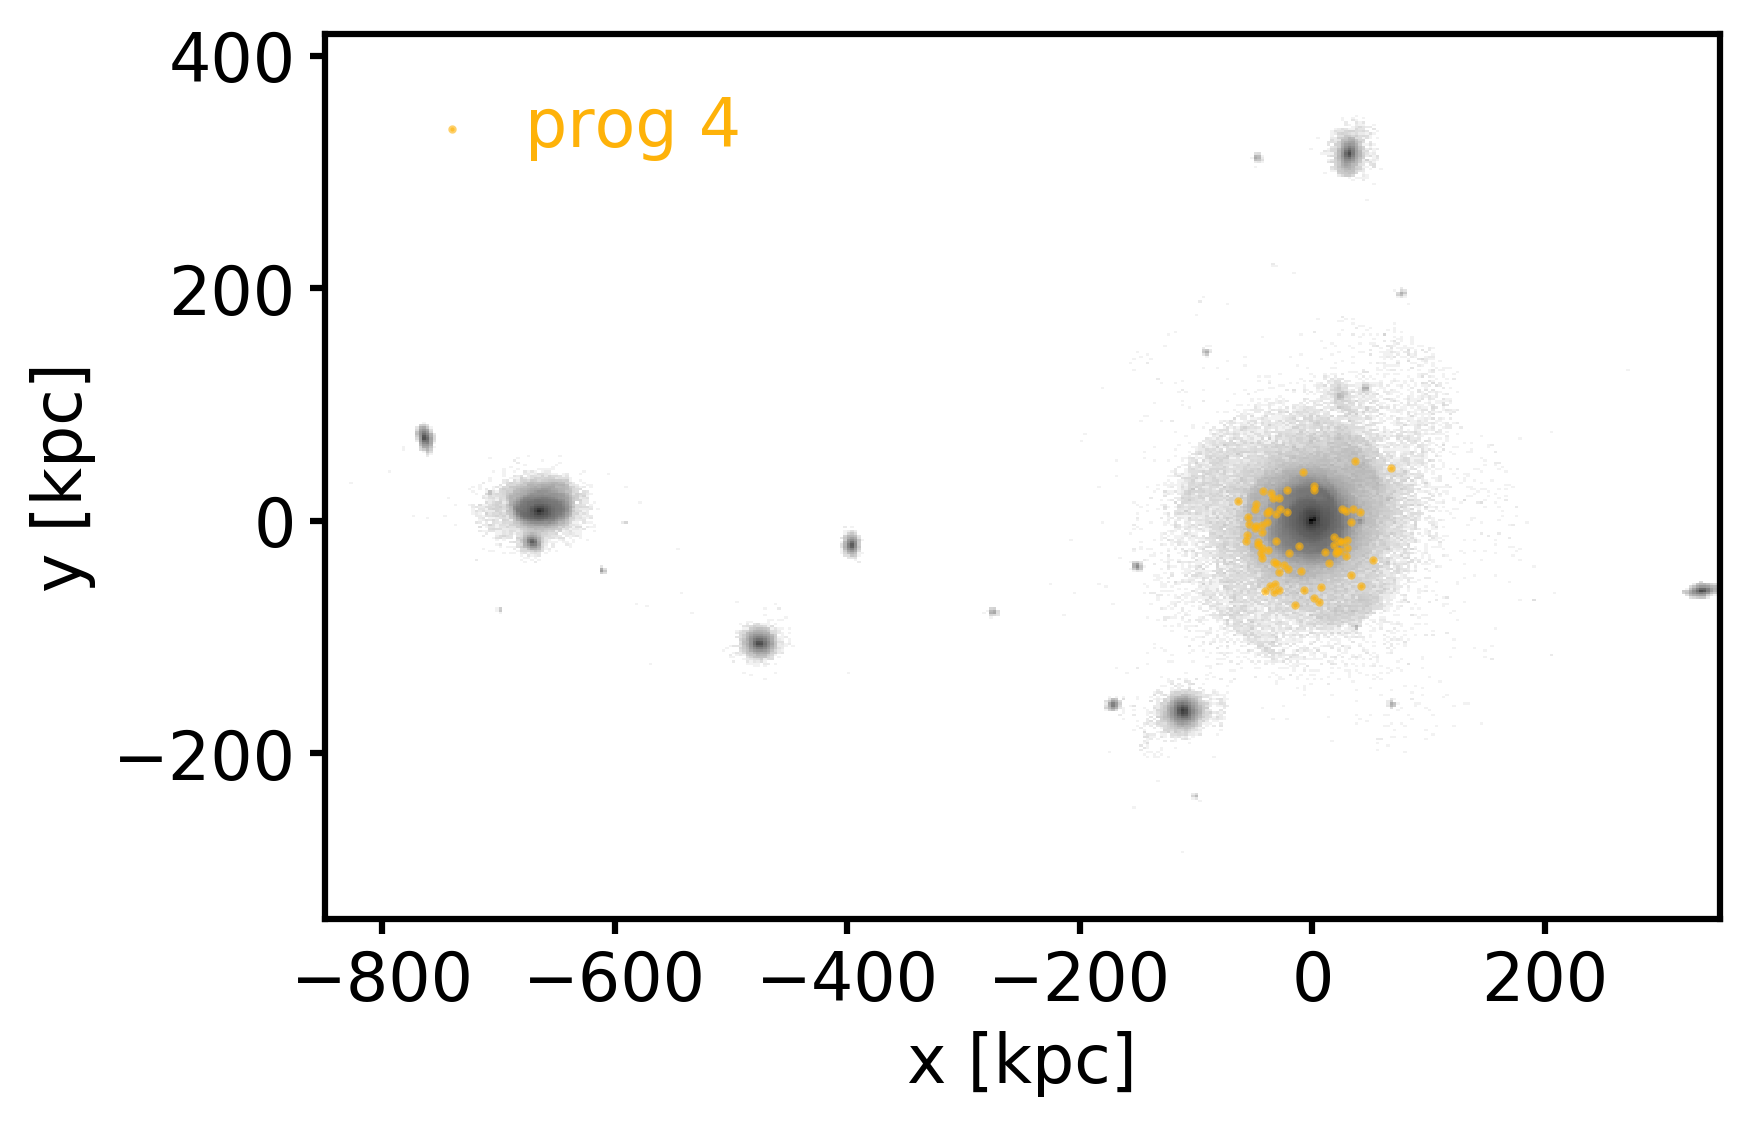
\includegraphics[width=\textwidth]{plots/Dynamics/dist/xy_dist_selected_GCs_prog_4_snap_127.png}
    	\label{fig:prog4_xy}
    \end{subfigure}
    ~ %add desired spacing between images, e. g. ~, \quad, \qquad, \hfill etc. 
    %(or a blank line to force the subfigure onto a new line)
    \begin{subfigure}[c]{0.45\textwidth}
        \centering
    	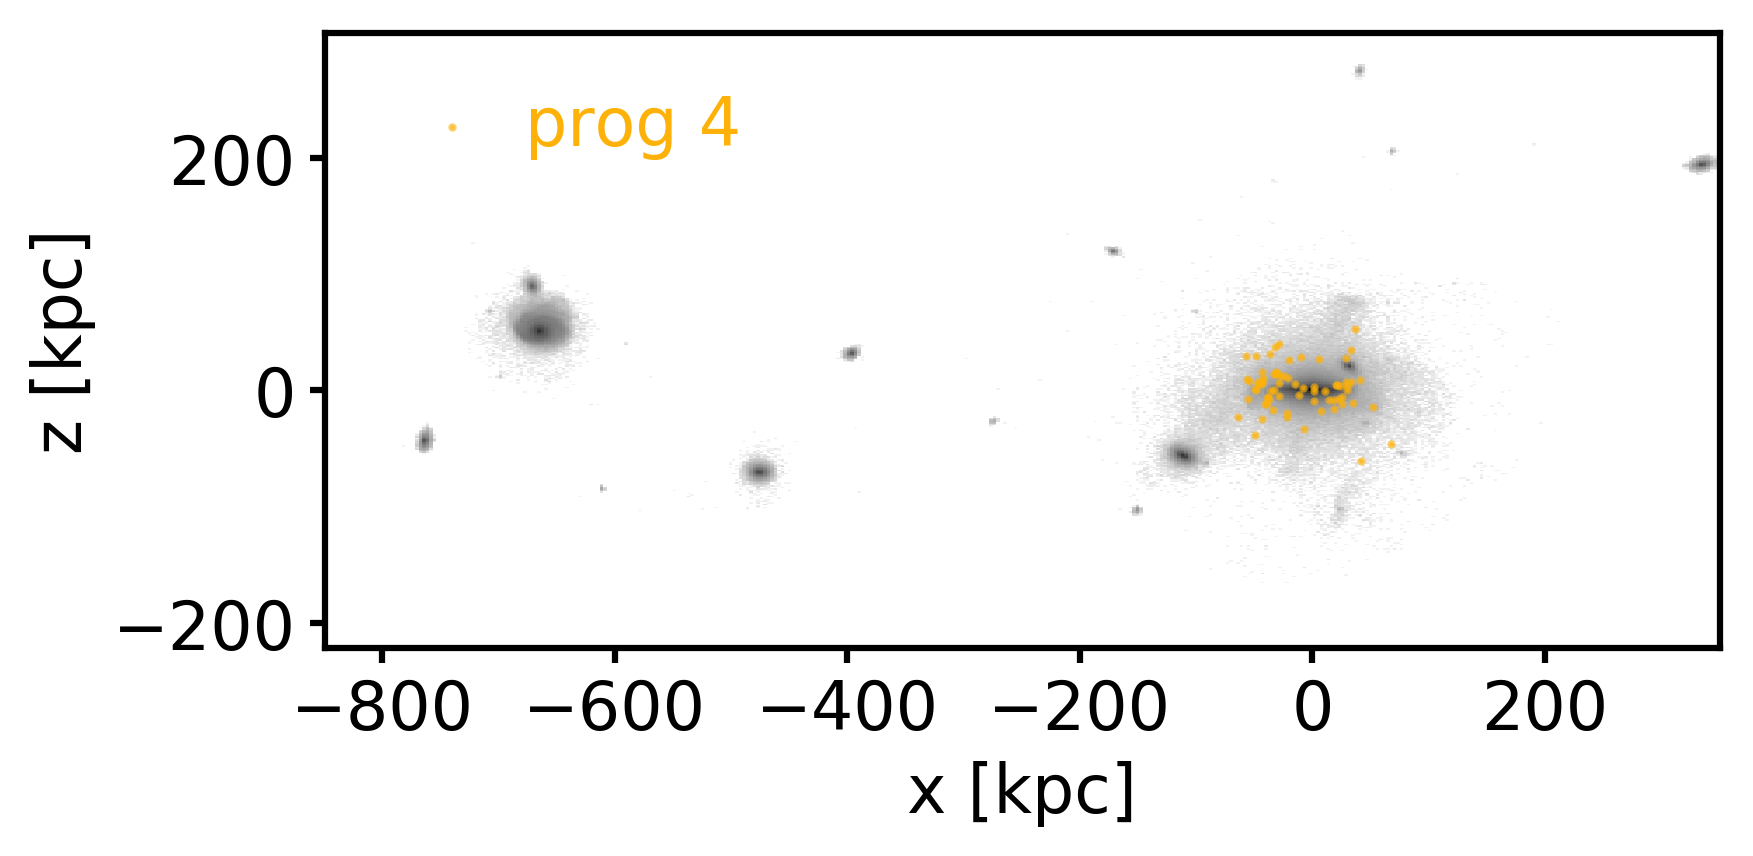
\includegraphics[width=\textwidth]{plots/Dynamics/dist/xz_dist_selected_GCs_prog_4_snap_127.png}
	    \label{fig:prog4_xz}
    \end{subfigure}
    \caption{.}\label{fig:progenitors_distribution}
\end{figure}


\subsection{Globular clusters in action space}
\subsubsection{Best fit potential}
\begin{figure}[htbp]
    \centering
    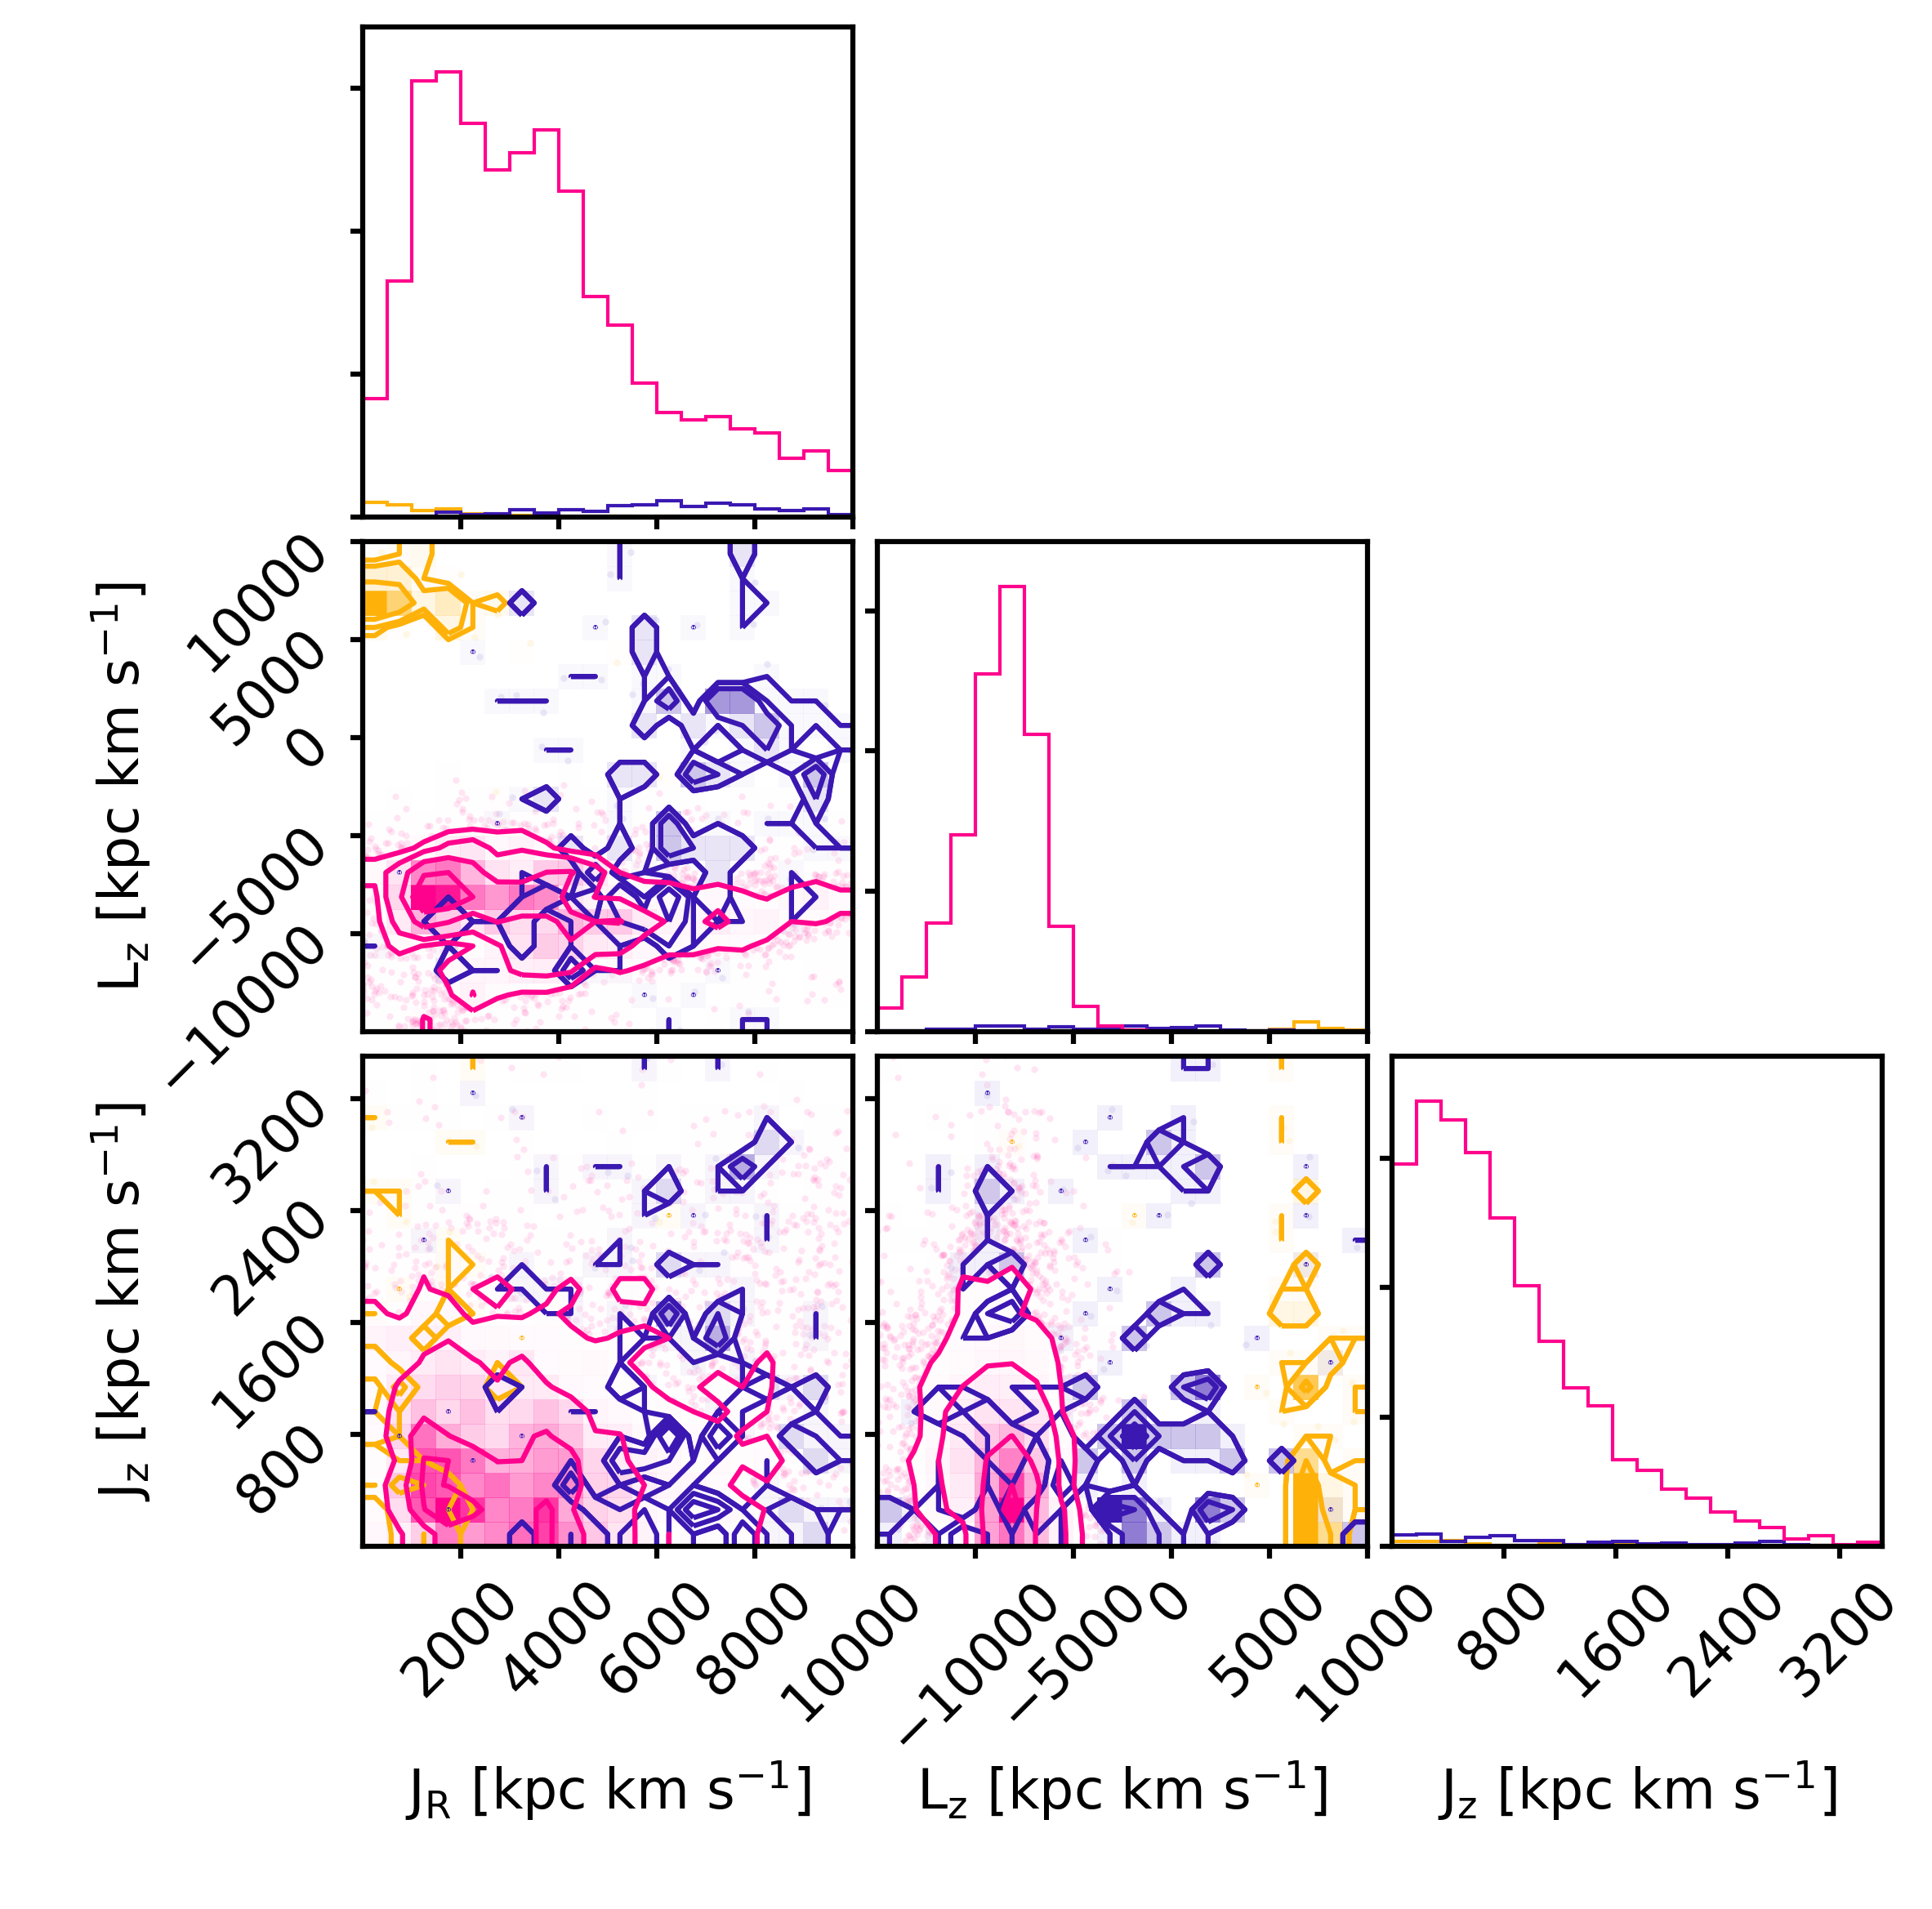
\includegraphics[width=1.0\textwidth]{plots/Dynamics/prog234_actions_snap_127.png}
    \caption{Selected \acp{GC} from three different \acp{DG} in action space.}
    \label{fig:act_both_merg_best_pot}
\end{figure}



\subsubsection{Varying potentials}

\begin{figure}[htbp]
    \begin{subfigure}[b]{0.45\textwidth}
    \centering
    	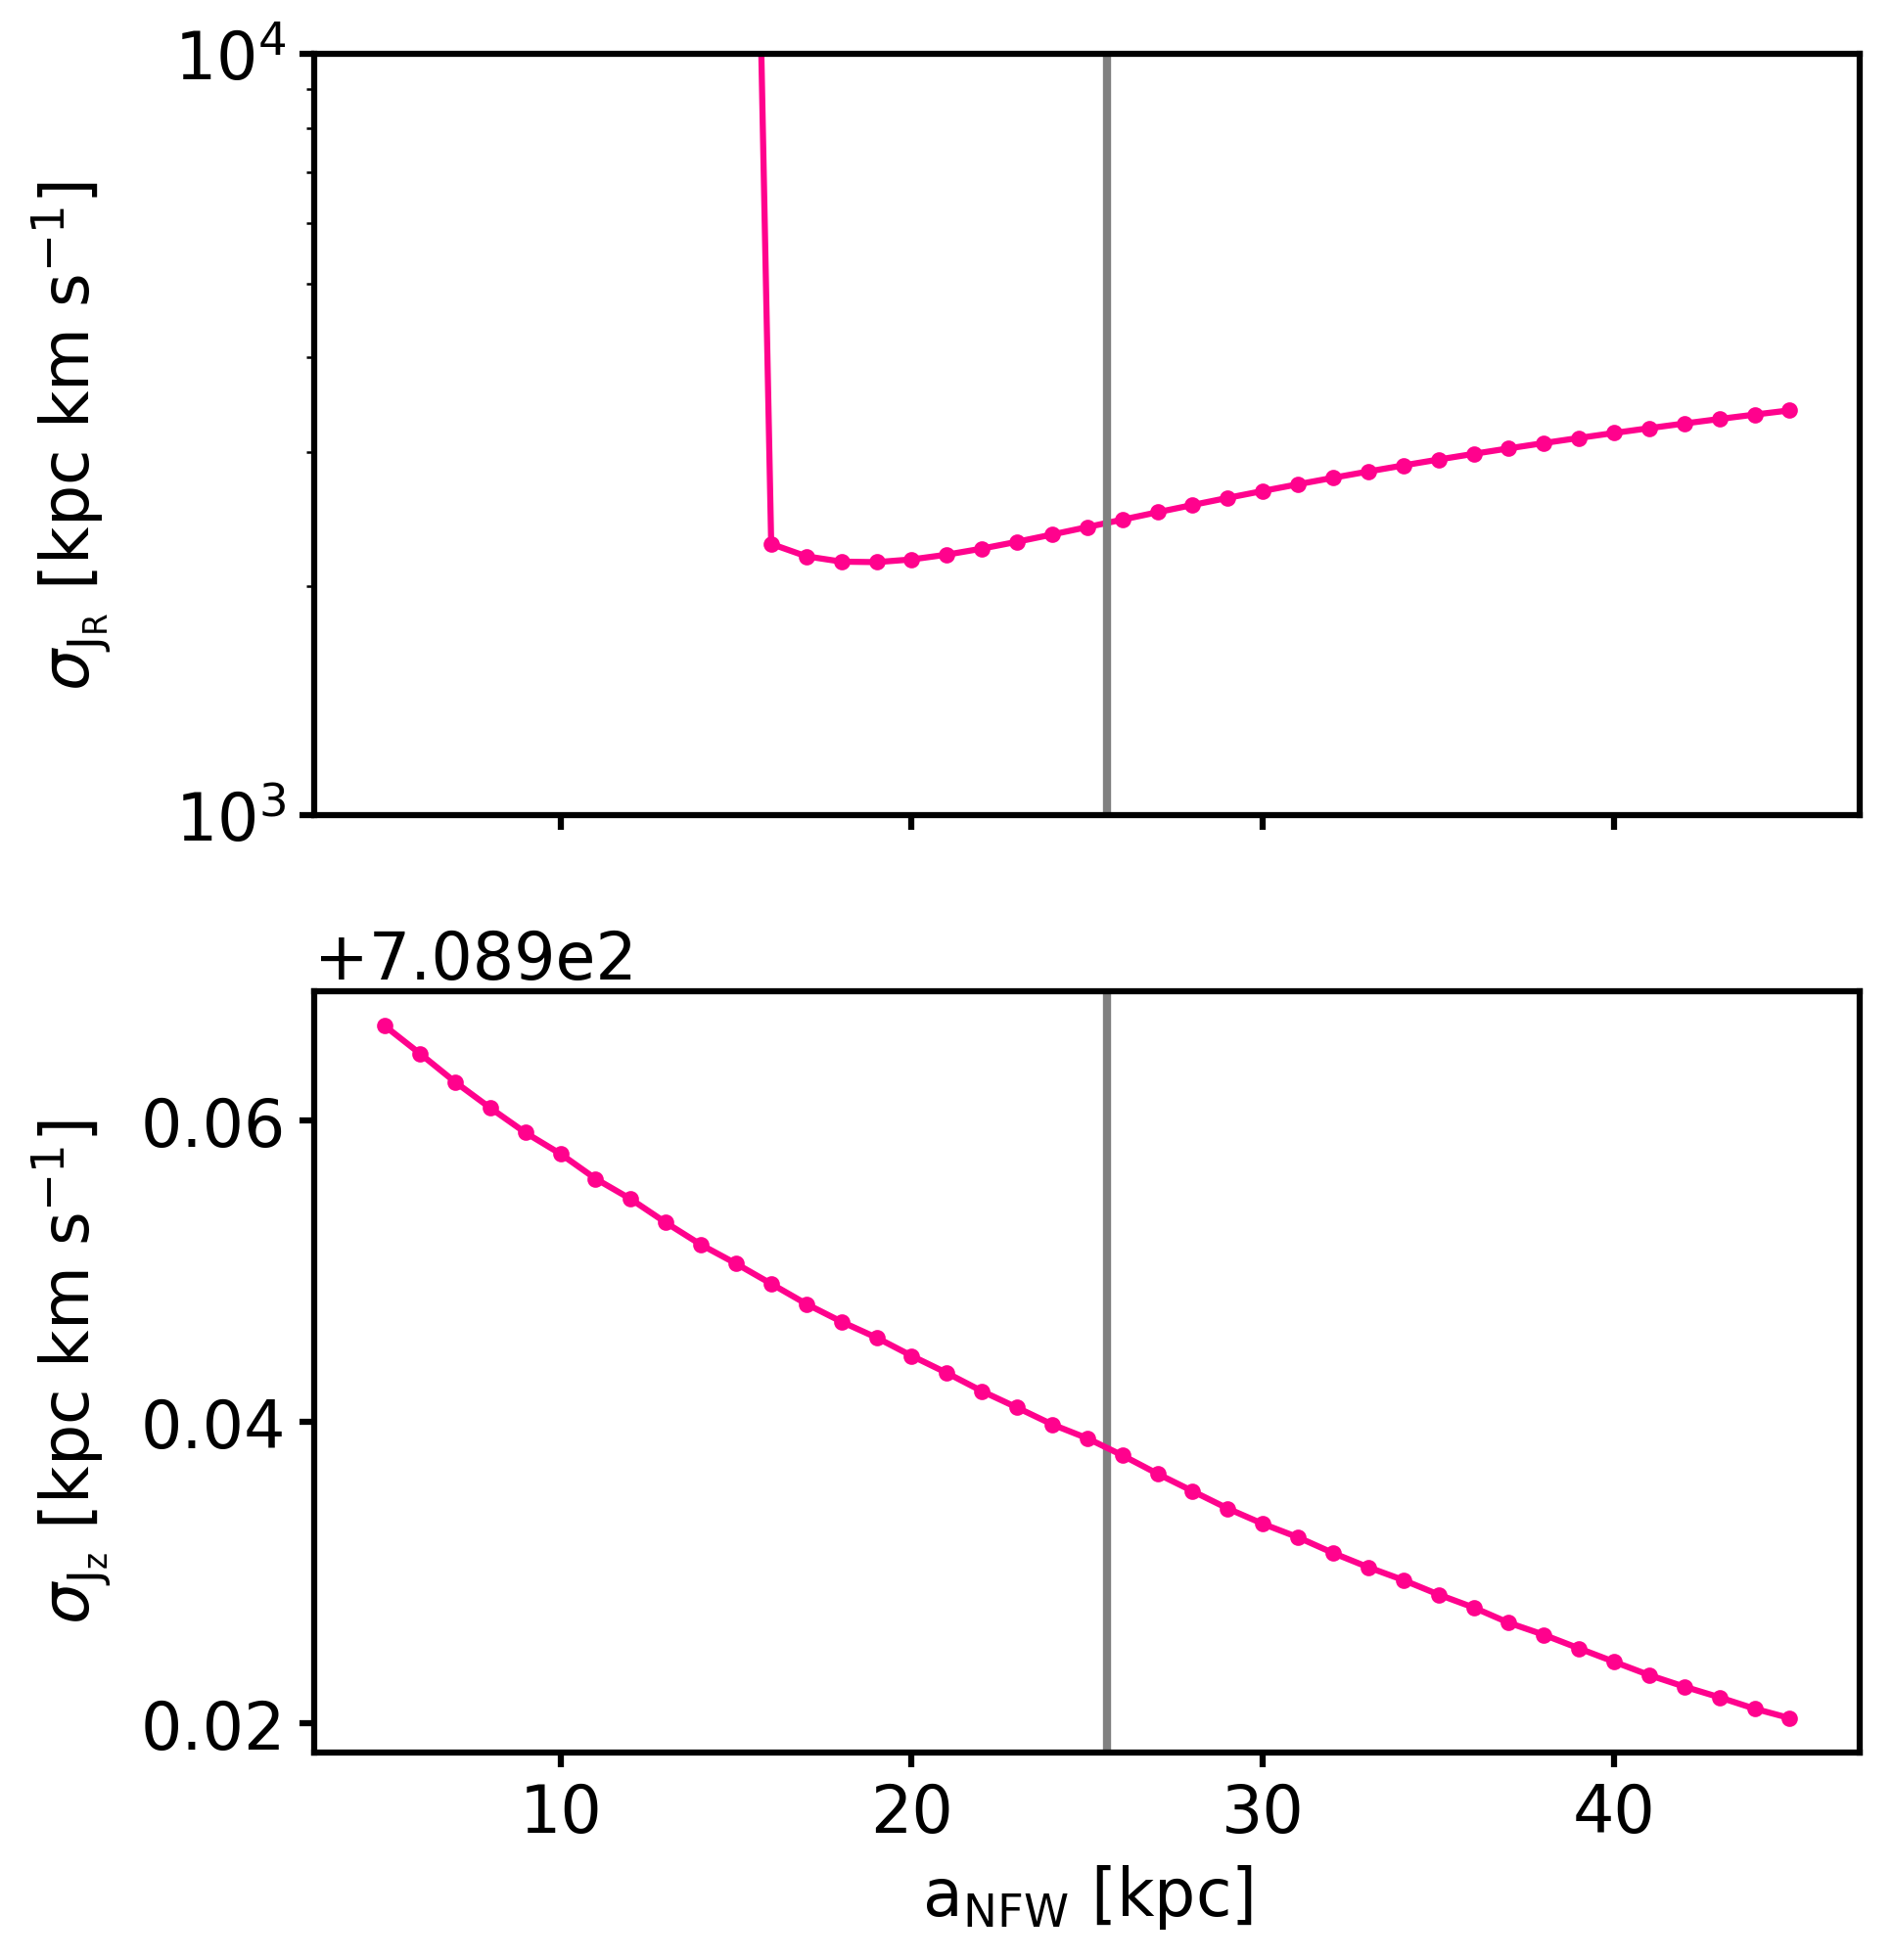
\includegraphics[width=\textwidth]{plots/Dynamics/prog2/a_NFW_diagnostic_plot_std_prog2_all.png}
    	\label{fig:NFW_diag_all_GCs}
    \end{subfigure}
    ~ %add desired spacing between images, e. g. ~, \quad, \qquad, \hfill etc. 
    %(or a blank line to force the subfigure onto a new line)
    \begin{subfigure}[b]{0.45\textwidth}
        \centering
    	\includegraphics[width=\textwidth]{plots/Dynamics/a_67_NFW_diagnostic_plot_std_small_box.png}
	    \label{fig:NFW_diag_box_GCs}
    \end{subfigure}
    \caption{Standard deviation of radial and vertical action in different potentials for all \acp{GC} vs box \acp{GC}.}\label{fig:NFW_diagnostics}
\end{figure}

\subsection{Time evolution of actions}
\begin{figure}[htbp]
    \begin{subfigure}[b]{0.5\textwidth}
    \centering
    	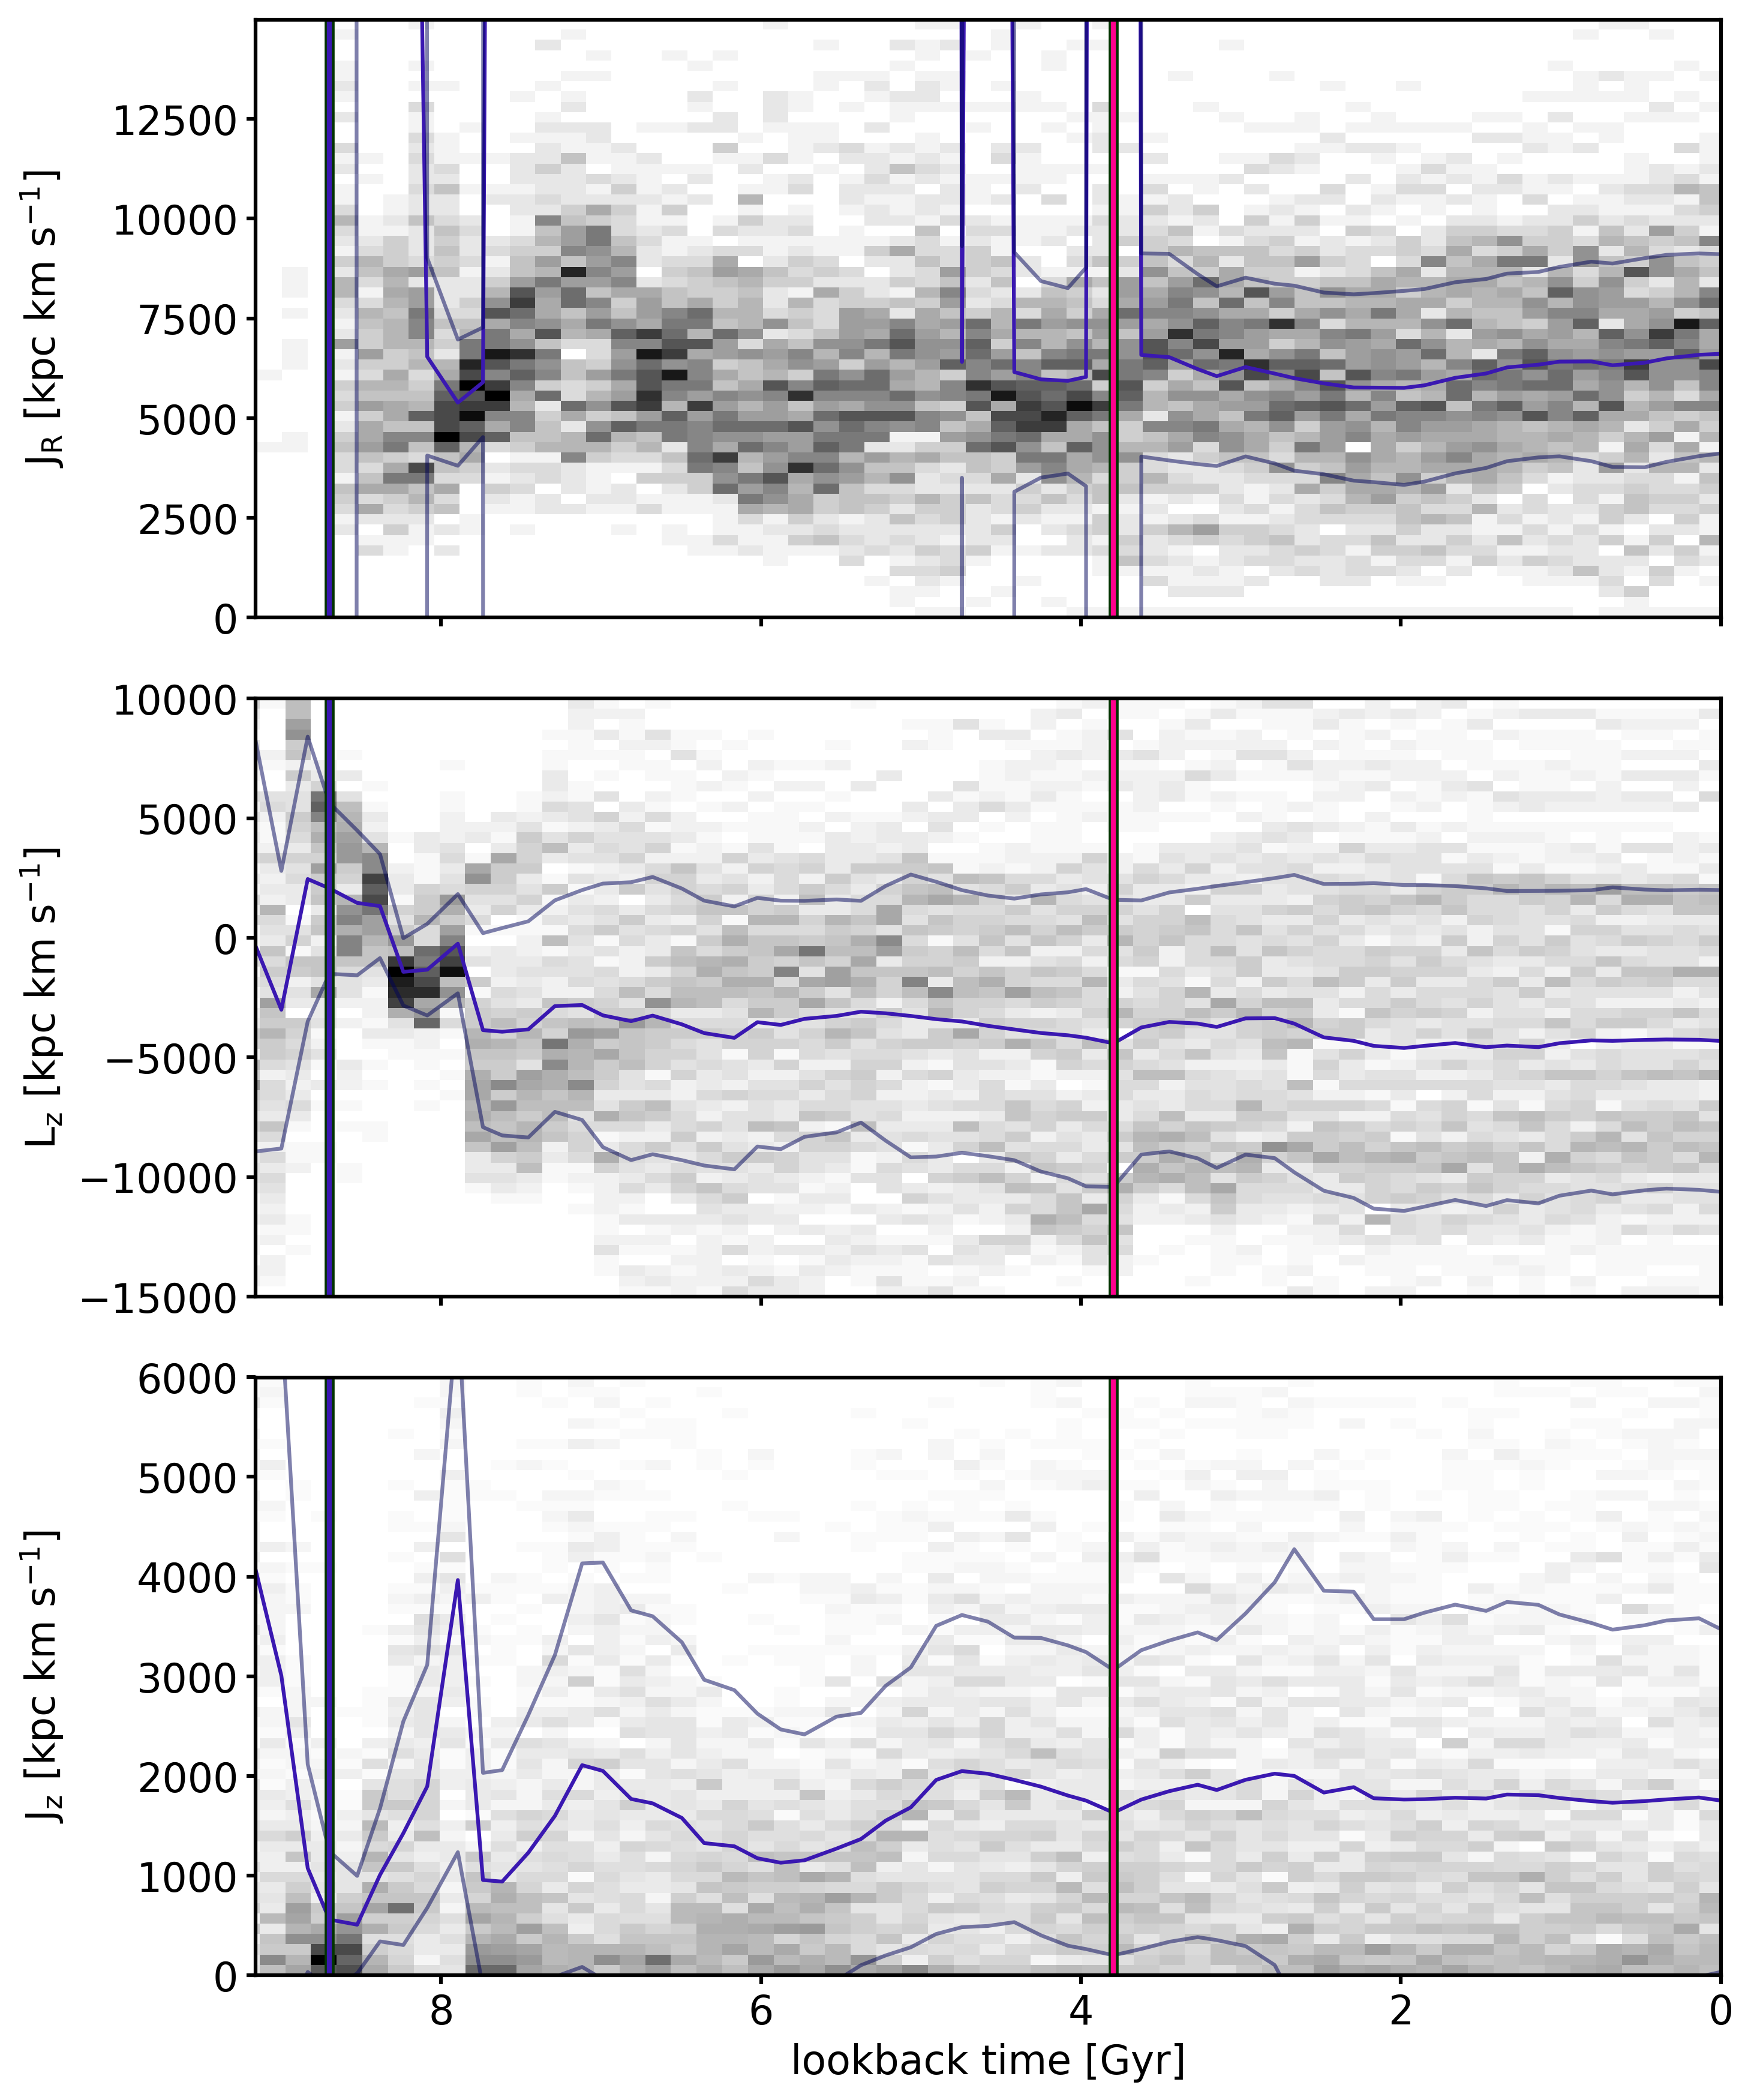
\includegraphics[width=\textwidth]{plots/Dynamics/action_time_evolution_hist_mean.png}
    	\label{fig:time_ev_all_GCs}
    \end{subfigure}
    \begin{subfigure}[b]{0.5\textwidth}
        \centering
    	\includegraphics[width=\textwidth]{plots/Dynamics/merger_67_small_box_action_evolution_with_errros.png}
	    \label{fig:time_ev_box_GCs}
    \end{subfigure}
    \caption{Time evolution of actions of all accreted \acp{GC} from one \ac{DG} vs. box selected sample.}\label{fig:actions_time_evolution}
\end{figure}
